% !TEX TS-program = pdflatexmk
\documentclass[12pt,a4paper,oneside,titlepage,pdftex]{article}
\usepackage[utf8]{inputenc}
\usepackage[T1]{fontenc}
%\usepackage[OT1]{fontenc}

\usepackage[english,finnish]{babel}

% Enable/disable MathTime fonts depending on if they are available
%\usepackage[T1,mtbold,lucidacal,mtplusscr,subscriptcorrection]{mathtime}

%\usepackage{times}
%\usepackage{fourier}
%\usepackage{lmodern}
%\usepackage{palatino}
%\usepackage{tgpagella}

\usepackage{hyphenat}

\usepackage[pdftex]{graphicx}
\usepackage{color}
\usepackage[pdftex,colorlinks=true,citecolor=black,
            pagecolor=black,linkcolor=black,menucolor=black,
            urlcolor=black]{hyperref}
\usepackage{eufrak}
\usepackage{amsmath}
\usepackage{amsbsy}
\usepackage{eucal}
%\usepackage{subfigure}

\usepackage{longtable}
\usepackage{url}
\urlstyle{same}

\usepackage{booktabs}
\usepackage{tabularx}
\usepackage{multicol}
\usepackage{multirow}
\usepackage{rotating}
\usepackage[margin=10pt,font=normalsize,labelfont=bf,labelsep=period]{caption}

% For pmatrix* (starred version which allows to specify alignment)
\usepackage{mathtools}

\usepackage[]{natbib}
\usepackage{graphicx,enumerate}
\bibliographystyle{plain}

\usepackage{url}
%% Define a new 'leo' style for the package that will use a smaller font.
\makeatletter
\def\url@leostyle{%
  \@ifundefined{selectfont}{\def\UrlFont{\sf}}{\def\UrlFont{\small\ttfamily}}}
\makeatother
%% Now actually use the newly defined style.
%\urlstyle{leo}

% Euro-merkki
%\usepackage{textcomp}
%\usepackage[official]{eurosym}
\usepackage[gen]{eurosym}

% Theorem env: http://www.maths.tcd.ie/~dwilkins/LaTeXPrimer/Theorems.html
\newtheorem{theorem}{Theorem}[section]
\newtheorem{lemma}[theorem]{Lemma}
\newtheorem{proposition}[theorem]{Proposition}
\newtheorem{corollary}[theorem]{Corollary}

\newtheorem{remark}[theorem]{Remark}
\newtheorem{example}[theorem]{Example}
\newtheorem{definition}[theorem]{Definition}

\newenvironment{proof}[1][Proof]{\begin{trivlist}
\item[\hskip \labelsep {\bfseries #1}]}{\end{trivlist}}
\newenvironment{motivation}[1][Motivation]{\begin{trivlist}
\item[\hskip \labelsep {\bfseries #1}]}{\end{trivlist}}

\newcommand{\qed}{\nobreak \ifvmode \relax \else
      \ifdim\lastskip<1.5em \hskip-\lastskip
      \hskip1.5em plus0em minus0.5em \fi \nobreak
      \vrule height0.75em width0.5em depth0.25em\fi}
% end of theorem env

\newcommand{\thedate}{\today}

% Commands for common sums
\newcommand{\Sumij}{\sum_{i,j=1}^n}
\newcommand{\Sumi}{\sum_{i=1}^n}

% Roman numerals
\makeatletter
\newcommand{\rmnum}[1]{\romannumeral #1}
\newcommand{\Rmnum}[1]{\expandafter\@slowromancap\romannumeral #1@}
\makeatother

% Try to prevent widow and orphan lines
\widowpenalty=300
\clubpenalty=300
\setlength{\parskip}{3ex plus 2ex minus 2ex}

%\setlength{\parskip}{1em}
\setlength{\parindent}{0em}

% SUOMI: Poikkeustavutuslista
\hyphenation{  }


% Headings using the fancyhdr package
\usepackage{fancyhdr}
\setlength{\headheight}{15pt}
\pagestyle{fancy}

\fancyhf{}
 
\lhead{Aineopintojen harjoitustyö: Tietokantasovellus}
\rhead{Vesa Riekkinen}
\rfoot{\thepage}

\pdfinfo{
          /Title      (582203 Aineopintojen harjoitustyö: Tietokantasovellus)
          /Author     (Vesa Riekkinen)
          /Keywords   ()
}

\title{Tehtävälista}
\date{4.4.2016}
\author{582203 Aineopintojen harjoitustyö: Tietokantasovellus\\ \\ Vesa Riekkinen\\ \\Helsingin yliopisto\\Matemaattis-luonnontieteellinen tiedekunta\\Tietojenkäsittelytiede}

%-------------------------------------------------------------------------------------------------------------------

\begin{document}

\maketitle

\setcounter{page}{1}
\pagenumbering{arabic}
 
\section{Johdanto}

Työn aihe on verkossa toimiva tehtävälista eli niin sanottu to do -lista. Sovelluksen käyttötarkoitus on, että käyttäjä voi kirjata sovellukseen tulevien päivien ja viikkojen tehtävät. Tämän tyyppisen sovelluksen tavoite on auttaa käyttäjiä heidän oman aikansa hallinnassa. Yksi perustavanlaatuinen syy tehtävälistan ylläpidolle on vähentää tehtävien järjestämisestä syntyvää aivojen kuormitusta kirjoittamalla ne esimerkiksi muistilapulle. Nykypäivänä lienee varsin luonnollista, että paperille kirjoitettujen muistilappujen lisäksi käytetään myös digitaalisia verkkopalveluita. Tämän tyyppisiä olemassa olevia verkkopalveluita ovat esimerkiksi todoist.com ja any.do.

Työn aihe on mukautettu versio valmiista aiheesta nimeltä Muistilista. Olennaisin ero valmiiseen aiheeseen verrattuna on, että tämä sovellus järjestää tehtävät etupäässä päivämäärän mukaan. Valmis aihe Muistilista vuorostaan järjestää tehtävät etupäässä niiden prioriteetin mukaan. Tämä sovellus tulee todennäköisesti tarjoamaan myös mahdollisuuden tehtävien prioriteettien asettamiseen, mutta tämä tulee olemaan enemmänkin lisäominaisuus. Pääasiallinen tarkoitus on pitää kirjaa tehtävistä niiden suunnitellun suorituspäivämäärän mukaan.

Sovellus toteutetaan Javalla käyttäen Java EE:n web-profiilia. Web-profiili tosin sisältää useita eri tekniikoita, joista tämä sovellus käyttää vain pientä osaa. Tämä sovellus käyttää nimenomaan Java Servlet ja JavaServer Pages (JSP) -tekniikoita. Näitä tekniikoita täydentämään on kehitetty myös useita erilaisia sovelluskehyksiä, mutta tässä työssä ei ole tarkoitus käyttää mitään tällaista sovelluskehystä.

Servlet-tekniikan käyttö edellyttää sitä tukevan HTTP-palvelimen käyttöä. Kevyemmän mallisia servlet container -palvelimia ovat esimerkiksi Apache Tomcat ja Jetty. Nämä palvelimet ovat myös siinä mielessä erityisiä, että niitä voidaan ajaa niin sanotussa embedded-tilassa. Embedded-tila tarkoittaa olennaisesti sitä, että jokaiselle sovellukselle osoitetaan oma paikallinen HTTP-palvelin. Tällöin yksi palvelinohjelmiston kopio suorittaa vain yhtä sovellusta. Tämä on vastakohta perinteiselle mallille, jossa yksi keskitetty sovelluspalvelin pyörittää suurta joukkoa erilaisia sovelluksia. Uudentyyppistä hajautettua mallia käytetään joissakin pilvipalveluissa, jotka tyypillisesti pilkkovat kunkin palvelinkoneen fyysisesti tarjoamat resurssit useampaan virtuaaliseen ympäristöön. Tässä työssä hyödynnetään erästä tällaista pilvipalvelua.

Sovelluksen julkinen versio toimitetaan kehityksen aikana säännöllisesti Heroku\hyp{}pilvipalveluun. Sovelluksen kotisivu on verkossa osoitteessa tlist.herokuapp.com. Heroku noudattaa edellä kuvattua hajautettua mallia, jossa kukin sovellus käynnistää oman palvelimensa. Palvelinohjelmiston voi siis valita vapaasti, mutta sen tulee pystyä toimimaan embedded-tilassa. Tässä työssä käytetään Apache Tomcat -sovelluspalvelinta, mutta sovellus lienee yhtä lailla yhtäsopiva Jettyn kanssa.

Sovelluksen tietokannaksi on valittu PostgreSQL. PostgreSQL on kurssimateriaalissa suositeltu valinta. Heroku ei myöskään tarjoa muuta tietokantaa ilmaisversiossaan. Sovellus on tarkoitus toteuttaa SQL-standardien mukaisella yhteensopivalla tavalla, mutta kussakin tietokannassa on tietyt erityispiirteensä. Tällainen erityispiirre on esimerkiksi PostgreSQL:n serial-tyyppi tietokantataulujen pääavaimille. Toisin sanoen sovellus olisi todennäköisesti siirrettävissä toiseen tietokantatyyppiin kohtuullisen pienellä vaivalla, mutta sellaisenaan se toimii vain PostgreSQL-tietokannalla.

Sovelluksen käyttäjille verkossa näkyvät sivut toteutetaan HTML- ja CSS-tekniikoilla. Sivujen rakentamisessa hyödynnetään Bootstrap-kirjastoa, joka sisältää suuren joukon valmiita käyttöliittymäkomponentteja. Useimmat Bootstrapin komponentit ovat siinä mielessä staattisia, että ne eivät käytä Javascript-tekniikkaa. Tässä työssä on tarkoitus hyödyntää staattisten komponenttien lisäksi myös muutamaa Bootstrapin Javascript-komponenttia. Siten käyttäjän selaimen on tuettava myös Javascriptiä, mikä on modernien selainten perusominaisuus.

\section{Yleiskuva järjestelmästä}

Sovellus ryhmittelee tehtävät sillä tavalla, että kukin tehtävä kuuluu johonkin projektiin. Projektin sisällä tehtäviä voi ryhmitellä edelleen sillä tavalla, että yhdellä tehtävällä voi olla alitehtäviä. Joka tapauksessa kullakin tehtävällä on sille osoitettu suorituspäivämäärä, jota voi tarpeen mukaan myös päivittää. Tehtäviä voi tarkastella sekä projektikohtaisesti että kootusti. Koottu näkymä näyttää tulevan päivän ja tulevan viikon tehtävät päiväkohtaisesti.

Järjestelmä on tarkoitettu yksittäisille käyttäjille. Järjestelmä ei siis tue tiimityöskentelyä. Tämä tarkoittaa, että kukin projekti voi kuulua vain yhdelle käyttäjälle. Toisin sanoen projektit, tunnisteet ja tehtävät ovat käyttäjäkohtaisia. Näitä tietoja ei voi jakaa muiden käyttäjien kanssa.

\begin{figure}[htb]
\begin{center}
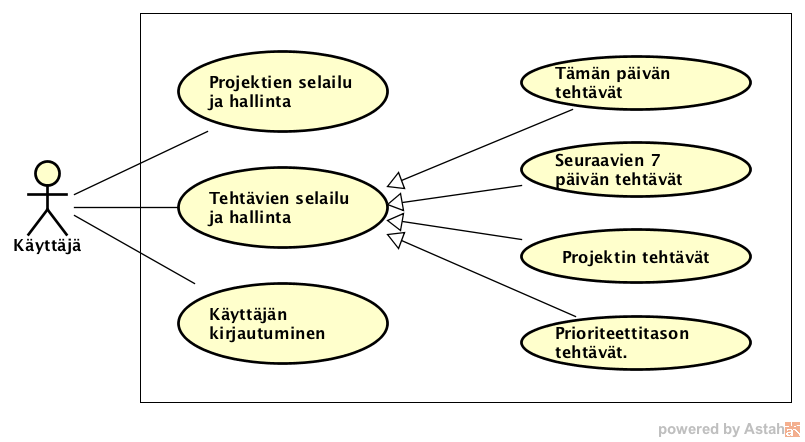
\includegraphics[width=\textwidth]{img/kayttotapauskaavio.png}
\caption{Käyttötapauskaavio}
\label{kasitekaavio}
\end{center}
\end{figure}

\section{Järjestelmän tietosisältö}

Järjestelmän tietosisältöä kuvaavia käsitteitä ovat käyttäjä, projekti, tunniste ja tehtävä. Järjestelmä toimii siten, että kullakin käyttäjällä on omat projektinsa, tunnisteensa ja tehtävänsä. Tässä järjestelmässä tehtävä on työn perusyksikkö, jolla on tietty päivämäärä. Tehtävät jaotellaan projekteihin. Tehtäviä voidaan luokitella myös yli projektirajojen käyttämällä tunnisteita.

Käyttäjällä voi olla mielivaltainen määrä projekteja ja tunnisteita. Kuhunkin projektiin ja kuhunkin tunnisteeseen voi liittyä mielivaltainen määrä tehtäviä. Projektilla ja tunnisteella on kuitenkin yksi keskeinen ero: yhdellä tehtävällä voi olla monta tunnistetta, mutta yksi tehtävä voi kuulua vain yhteen projektiin. Yksi tehtävä ei siis voi kuulua kahteen eri projektiin. Tehtävällä voi kuitenkin olla useita tunnisteita. Tehtävän tulee myös kuulua johonkin projektiin, mutta tunnisteiden merkitseminen on vapaaehtoista.

\begin{figure}[htbp]
\begin{center}
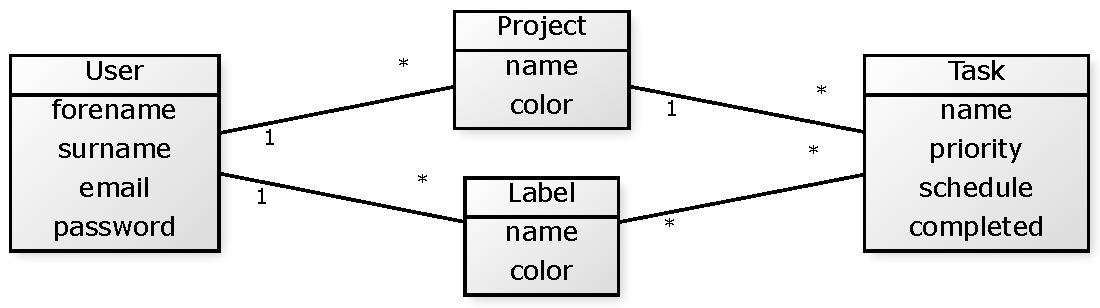
\includegraphics[width=\textwidth]{img/kasitekaavio.pdf}
\caption{Käsitekaavio}
\label{kasitekaavio}
\end{center}
\end{figure}

\begin{table}[htbp]
\renewcommand{\arraystretch}{1.2}
\caption{Järjestelmän tietokohteiden kuvaukset}
\makebox[\textwidth][c]{
\begin{tabularx}{1.15\textwidth}{lllX}
\toprule
Käsite & Attribuutti & Arvojoukko & Kuvaus \\
\midrule
Person &
forename    & Merkkijono (max 50)  & Käyttäjän etunimi      \\ 
& surname     & Merkkijono (max 50)  & Käyttäjän sukunimi    \\ 
& email         & Merkkijono (max 30)  & Käyttäjän sähköpostiosoite   \\ 
& password    & Merkkijono (max 100) & Käyttäjän salasanan tiiviste \\
\midrule
Project &
name    & Merkkijono (max 100) & Projektin nimi \\
& color     & Kokonaisluku            & Projektille asetettu RGB\hyp{}värikoodi \\
\midrule
Label &
name    & Merkkijono (max 100) & Tunnisteen nimi \\
& color     & Kokonaisluku            & Tunnisteelle asetettu RGB\hyp{}värikoodi \\
\midrule
Task &
name         & Merkkijono (max 250)  & Tehtävän nimi      \\ 
& priority      & Kokonaisluku            & Kokonaisluku välillä 1-4.    \\ 
& schedule     & Päivämäärä              & Suunniteltu suorituspäivä   \\ 
& completed   & Totuusarvo              & Kertoo onko tehtävä suoritettu \\
\bottomrule
\end{tabularx}
}
\end{table}

Käyttäjän salasanan tiiviste on merkkijono. Kenttä \emph{password} sisältää merkkijonon, joka voidaan välittää salasanoja käsittelevälle metodille sellaisenaan. Merkkijono sisältää varsinaisen salasanan tiivisteen lisäksi niin sanotun suolan ja muita toteutuksen tallentamia parametreja. Merkkijonon tarkka sisältö riippuu käytettävästä salausmoduulista.

Tehtävän prioriteetti on kokonaisluku välillä 1-4. Suurinta prioriteettia merkitään luvulla 1 ja pienintä prioriteettia luvulla 3. Jos prioriteettia ei ole asetettu lainkaan, sen arvoa merkitään luvulla 4. Prioriteetti on siis sitä suurempi, mitä pienempi sen lukuarvo on, ja asteikon nollakohta on luku 4.

Käyttäjä voi valita kullekin projektille ja tunnisteelle oman värin, jota käytetään käyttöliittymässä. Värit tallennetaan RGB-muodossa. Värikomponentit tallennetaan yhtenä kokonaislukuna, mikä on yleisesti käytetty tapa. Punainen, vihreä ja sininen komponentti tallennetaan bitteihin 1-24, 8 bittiä per värikomponentti.

\section{Relaatiotietokantakaavio}

Tietokantakaavio voidaan johtaa käsitekaaviosta lisäämällä kuhunkin tauluun pääavain, ja esittämällä yhteydet vierasavainten avulla. Tunnisteen ja ja tehtävän välillä on monesta\hyp{}moneen\hyp{}tyyppinen yhteys, jonka esittämiseen tarvitaan lisäksi yksi välitaulu.

\begin{figure*}[htbp]
\begin{center}
\makebox[\textwidth][c]{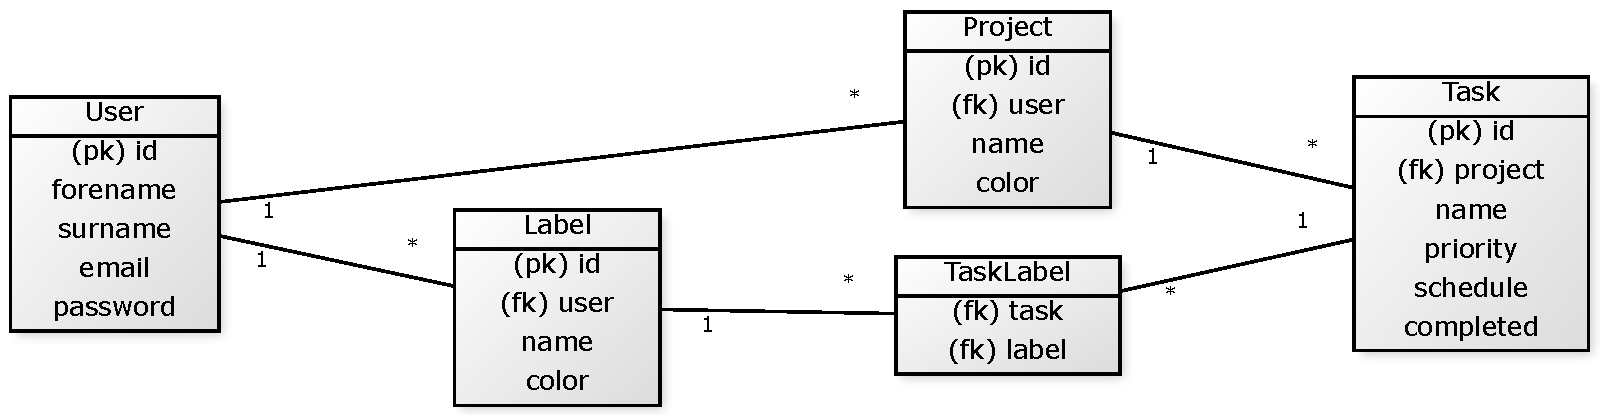
\includegraphics[width=1.3\textwidth]{img/tietokantakaavio.pdf}}
\caption{Tietokantakaavio}
\label{tietokantakaavio}
\end{center}
\end{figure*}

\section{Käynnistys-/käyttöohje}

Sovellus on asennettu Herokun pilvipalveluun. Sovellus löytyy osoitteesta

\begin{center}\url{http://tlist.herokuapp.com}\end{center}

Kirjautumista ei ole vielä toteutettu, joten sovellus avautuu oletuskäyttäjän tunnuksilla.

Projekteja voi selata vasemman reunan sivupalkista. Projektiin kuuluvat tehtävät saa näkyville klikkaamalla projektin nimeä. Projektin tehtävien listauksessa on toiminnot myös tehtävien lisäämiseen ja muokkaamiseen. Nappi tehtävän luomiseen on tehtävälistauksen alapuolella. Tehtävän muokkaaminen ja lisääminen tapahtuvat erillisen dialogin kautta. Dialogissa on nappi myös tehtävän poistamiseen.

\end{document}


%%% Local Variables: 
%%% mode: latex
%%% TeX-master: t
%%% End: 
